\section{Modelli utilizzati}
I tre modelli selezionati per la sperimentazione di questa tesi (YOLOv8, YOLO-World e RT-DETR) rappresentano l'avanguardia nell'ambito dell'Object Detection. Ognuno di essi presenta caratteristiche uniche che li rendono adatti a diversi scenari applicativi, rappresentando un ulteriore sviluppo rispetto alle precedenti iterazioni dei modelli YOLO.

\subsection{YOLOv8}
YOLOv8 rappresenta l'ultima evoluzione della famiglia YOLO, sviluppata da Ultralytics e rilasciata nel 2023\cite{26}. Questa versione introduce una serie di miglioramenti significativi rispetto alle precedenti, rendendolo uno degli algoritmi di rilevamento degli oggetti più avanzati e performanti disponibili oggi.

\subsubsection{Miglioramenti introdotti}
YOLOv8 introduce le seguenti migliorie: 
\begin{itemize}
  \item \textbf{Architettura Backbone}: YOLOv8 utilizza un'architettura backbone più avanzata che combina convolutional layers ottimizzati con tecniche di normalizzazione e attivazione migliorate, progettata per massimizzare l'estrazione delle feature mantenendo un alto livello di efficienza computazionale.
  \item \textbf{Residual Blocks e Dense Connections}: l'introduzione di residual blocks (simili a quelli di ResNet) e dense connections (ispirate a DenseNet) contribuisce a una migliore propagazione del gradiente durante l'addestramento. Vengono ridotti problemi come il vanishing gradient e migliorata la capacità della rete di apprendere rappresentazioni complesse, permettendo alla rete di addestrarsi.
  \item \textbf{GIoU Loss}: la loss function è stata migliorata con l'introduzione della Generalized Intersection over Union (GIoU) loss, la quale tiene conto non solo della sovrapposizione tra le bounding box previste e quelle reali, ma anche della distanza tra di esse.
  \item \textbf{Miglioramenti nelle FPN}: le feature pyramid networks sono state potenziate per fornire una migliore rappresentazione multi-scala delle feature dell'immagine, fattore che aiuta il modello a rilevare oggetti di diverse dimensioni, specialmente quelli piccoli.
  \item \textbf{Inferenza Accelerata}: grazie a ottimizzazioni specifiche nell'architettura e nell'implementazione del codice, YOLOv8 è in grado di eseguire l'inferenza a velocità superiori rispetto ai suoi predecessori.
  \item \textbf{Efficienza Computazionale}: la struttura generala è stata ottimizzata per essere eseguita su dispositivi con risorse limitate, come i dispositivi edge e embedded. 
  %Ciò rende YOLOv8 una scelta eccellente per applicazioni che devono girare su hardware a bassa potenza, come droni, telecamere di sicurezza e altri dispositivi IoT.
\end{itemize}

\begin{figure}[ht]
    \centering
    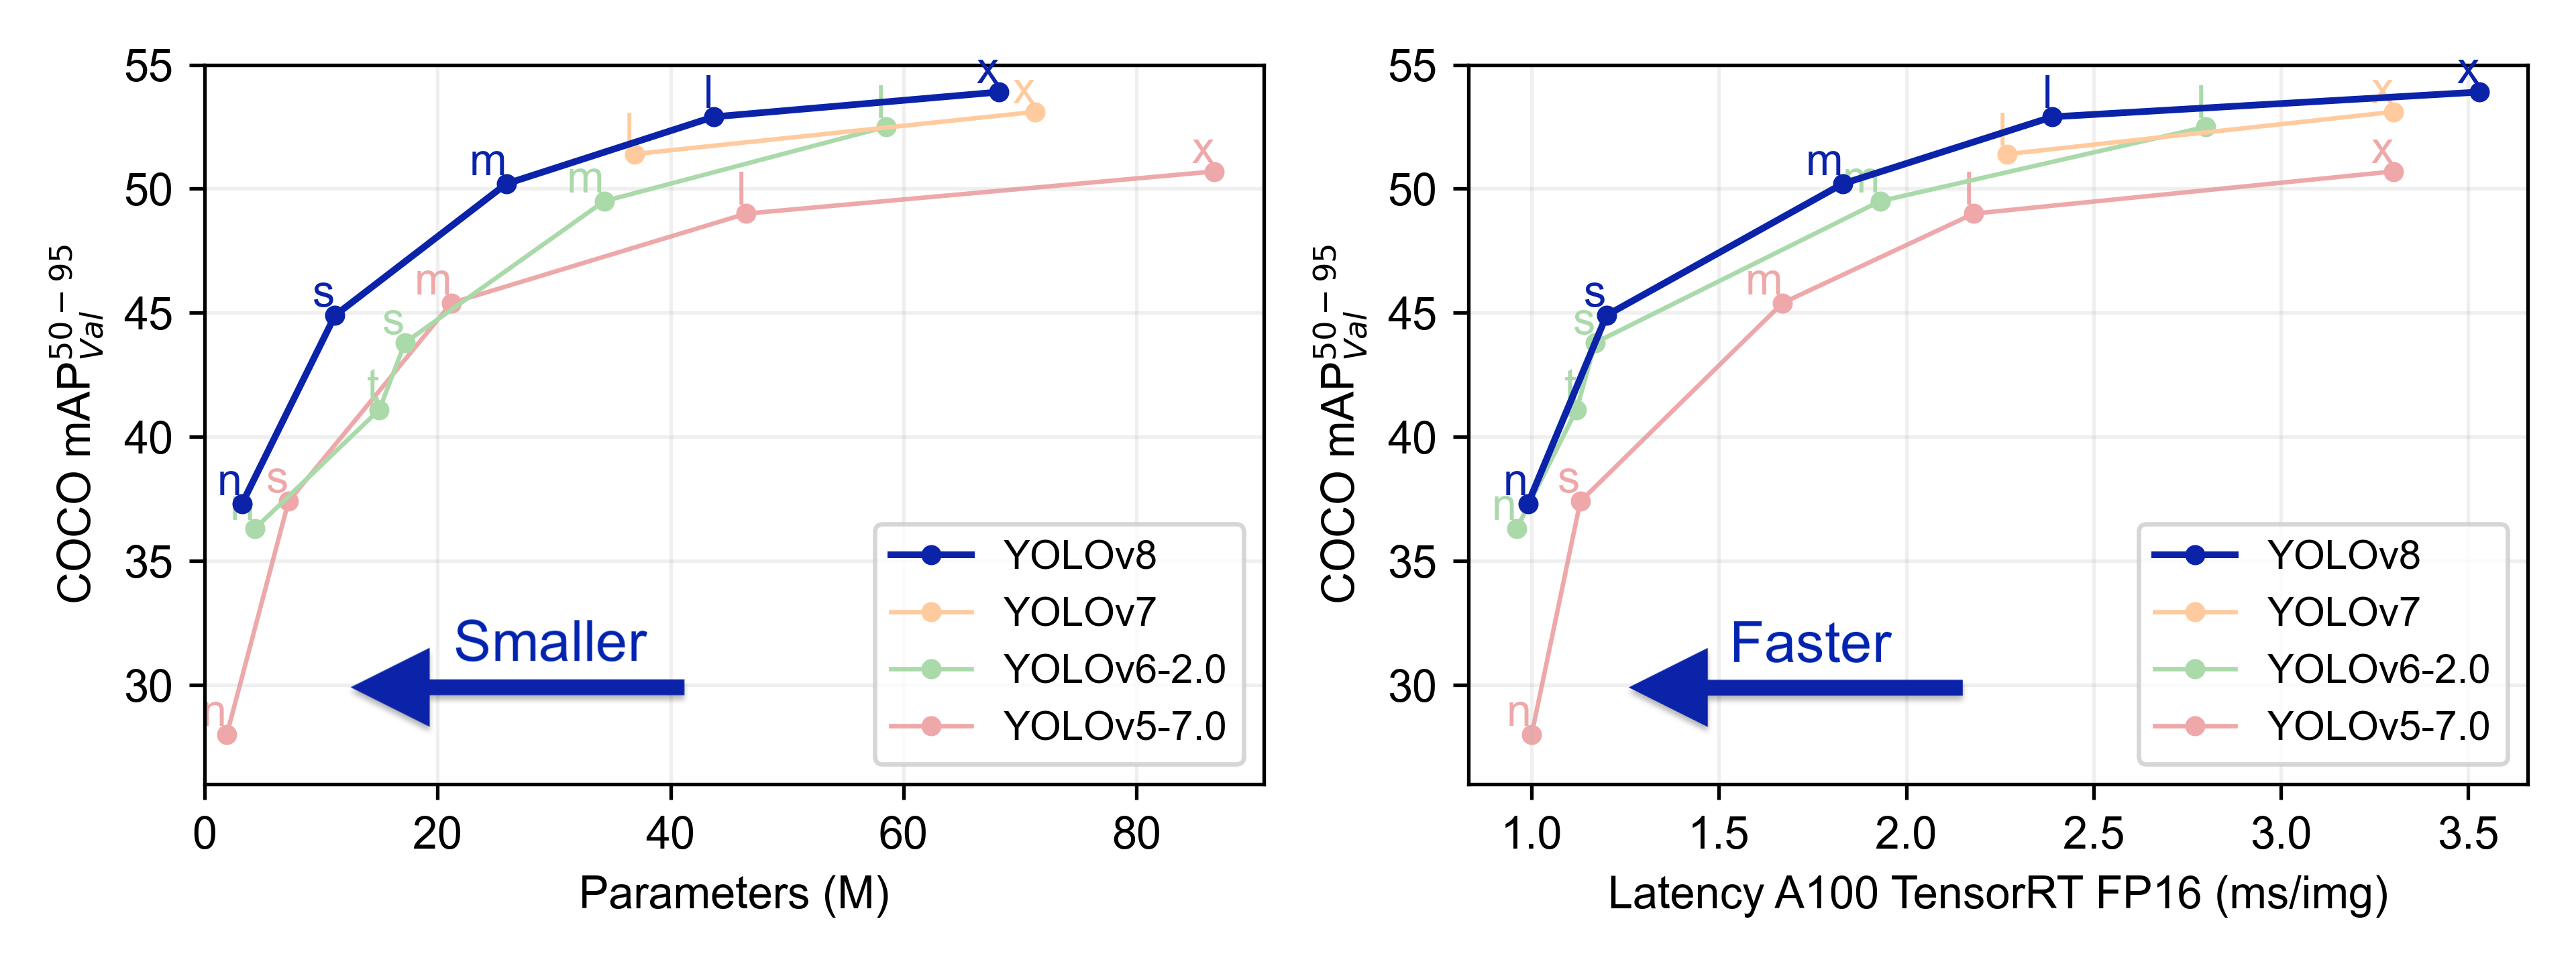
\includegraphics[width=0.95\textwidth]{files/capitoli/2-yolo/assets/yolov8-benchmark.png}
    \caption{\label{fig:yolov8-benchmark}mAP ottenuta da YOLOv8 su dataset COCO confrontata con quelle delle precedenti versioni\cite{27}}
\end{figure}

\newpage

\subsubsection{Architettura}
L'architettura di YOLOv8 si suddivide in 3 blocchi principali:
\begin{itemize}
  \item \textbf{Backbone}: chiamato anche Feature Extractor, è responsabile dell'estrazione delle feature significative dall'input. Nei suoi strati iniziali, rileva schemi semplici come bordi e texture, e man mano che si avanza, il backbone rileva feature a più scale, ottenendo rappresentazioni a diversi livelli di astrazione.
  \item \textbf{Neck}: funge da ponte tra il Backbone e il blocco successivo (Head). Esso costruisce piramidi di feature aggregando le feature maps ottenute dal backbone ed eseguendo la concatenazione o fusione di feature a diverse scale per garantire che la rete possa rilevare oggetti di diverse dimensioni. Inoltre, integra informazioni contestuali per migliorare l'accuratezza del rilevamento e riduce la risoluzione spaziale e la dimensionalità delle risorse per facilitare il calcolo, aumentando la velocità.
  \item \textbf{Head}: è la parte finale dell'architettura e si occupa di generare gli output della rete. Genera le bounding boxes associate ai possibili oggetti nell'immagine, assegna punteggi di confidenza a ciascuna bounding box per indicare la probabilità della presenza di un oggetto, e classifica gli oggetti nelle bounding boxes in base alle loro categorie.
\end{itemize}

\newpage

\begin{figure}[ht]
    \centering
    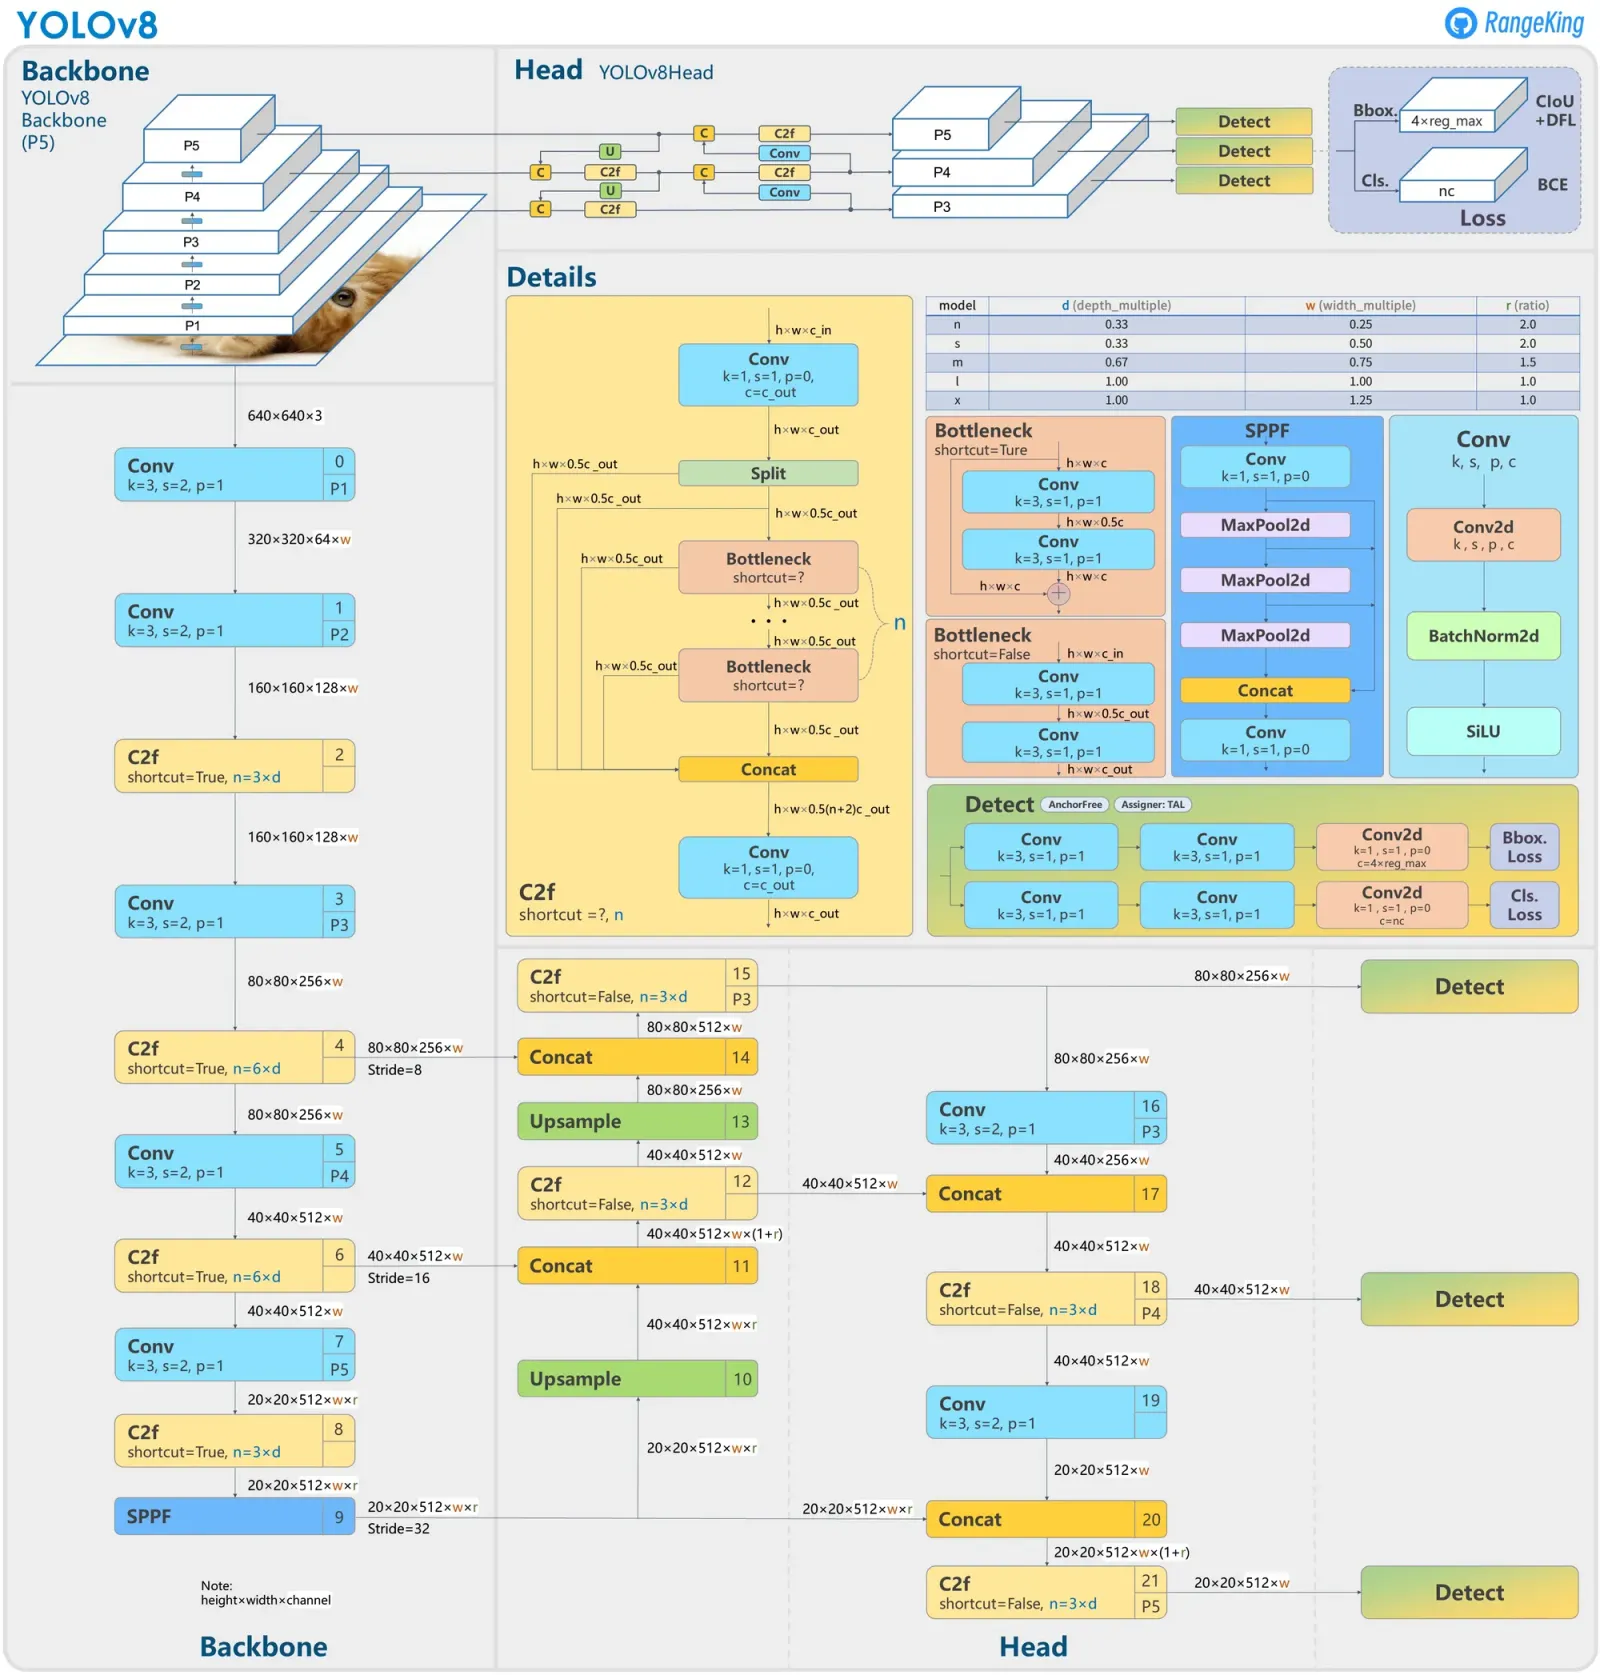
\includegraphics[width=1\textwidth]{files/capitoli/2-yolo/assets/yolov8-architecture.png}
    \caption{\label{fig:yolov8-architecture}Architettura di YOLOv8\cite{28}}
\end{figure}

\newpage

\subsection{YOLO-World}
YOLO-World è una recente evoluzione della famiglia di algoritmi YOLO\cite{29}, rivoluzionaria nella open-vocabulary object detection, che combina efficacemente l'efficienza di YOLOv8 con la potenza della modellazione vision-language ed un massiccio pre-training.

\subsubsection{Open-Vocabulary Object Detection}
L'object detection open-vocabulary (OVD) si propone di rilevare qualsiasi oggetto descritto tramite linguaggio naturale, anche se non è stato "visto" durante l'addestramento, superando così le limitazioni dei detector tradizionali che si concentrano su categorie di oggetti fissate.

YOLO-World in particolare consente di specificare dinamicamente le classi tramite prompt personalizzati, permettendo così agli utenti di adattare il modello alle proprie esigenze  senza doverlo addestrare nuovamente. Questa caratteristica è particolarmente utile per adattare il modello a nuovi domini o compiti specifici che non erano originariamente parte dei dati di addestramento. Impostando prompt personalizzati, gli utenti possono guidare il focus del modello verso gli oggetti di interesse, migliorando l'accuratezza dei risultati di detection.

\vspace{1cm}

\begin{figure}[ht]
    \centering
    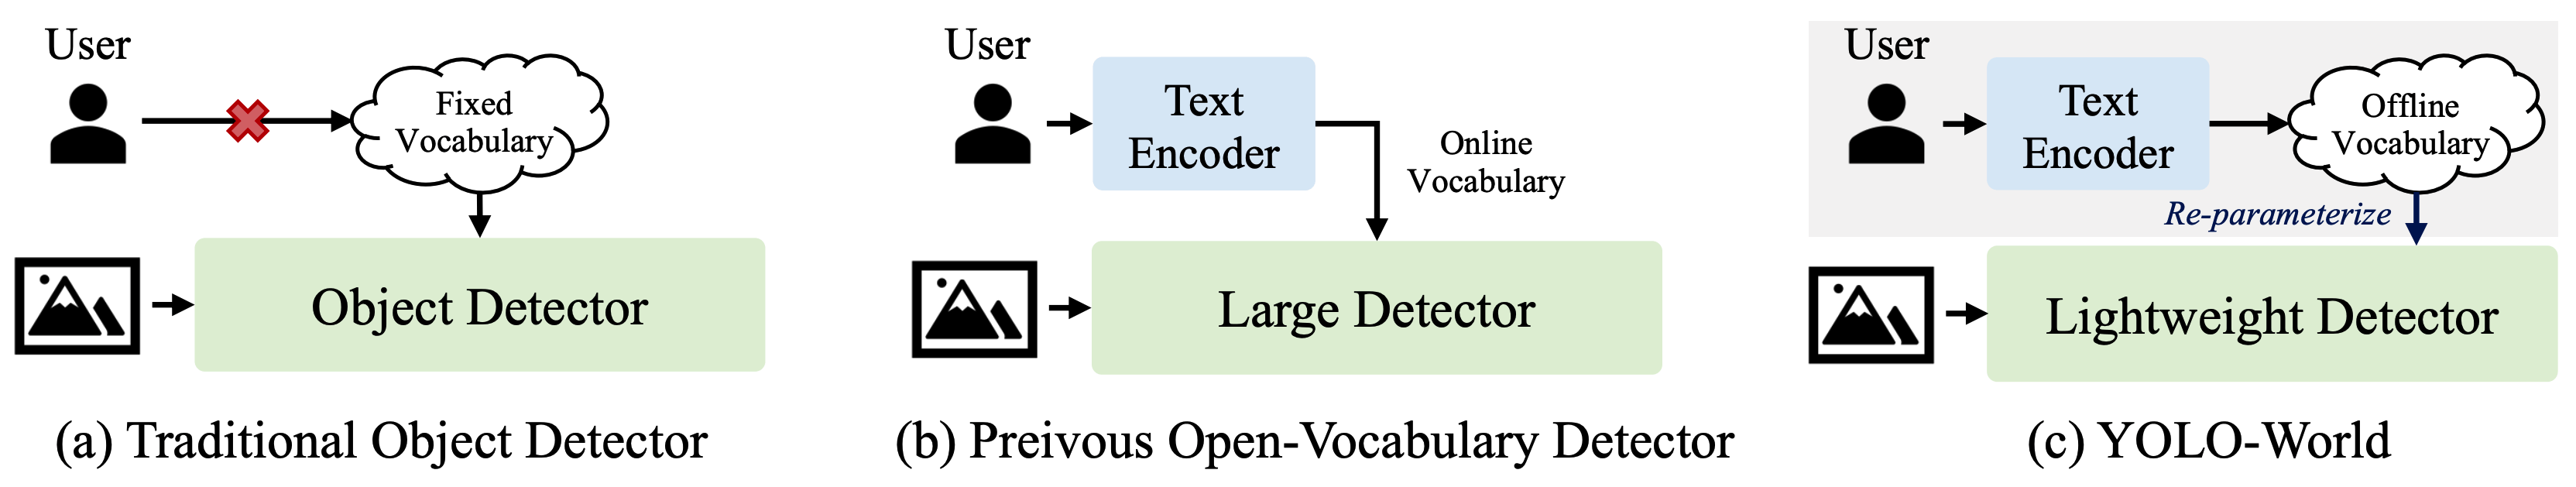
\includegraphics[width=1\textwidth]{files/capitoli/2-yolo/assets/yoloworld-ovd.png}
    \caption{\label{fig:yoloworld-ovd}Open-Vocabulary Object Detection di YOLO-World\cite{30}}
\end{figure}

\subsubsection{Innovazioni introdotte}
YOLO-World introduce le seguenti innovazioni:
\begin{itemize}
  \item \textbf{Paradigma Prompt-Then-Detect}: precomputando vocabolari offline basati su prompt definiti dall'utente, YOLO-World evita la necessità di codifica del testo in tempo reale, migliorando la velocità di inferenza e semplificando la personalizzazione.
  \item \textbf{Vision-Language Grounding}: la capacità del modello di comprendere e correlare informazioni visive con descrizioni in linguaggio naturale porta a rilevazioni più precise e consapevoli del contesto.
  \item \textbf{Ridotta Complessità del Modello}: la sua architettura evita le pesanti componenti basati su Transformer presenti nei modelli OVD precedenti, promuovendo l'accessibilità.
  \item \textbf{Etica Open-Source}: rilasciato sotto la GPL (General Public License), favorisce la collaborazione, accelera l'innovazione e garantisce che la tecnologia rimanga accessibile alla comunità più ampia.
\end{itemize}

\subsubsection{Architettura}
Le componenti principali dell'architettura di YOLO-World:
\begin{itemize}
  \item \textbf{YOLOv8 Backbone}: si occupa dell'estrazione delle feature, fornendo dettagliate rappresentazioni multi-scala delle immagini in input.
  \item \textbf{Text Encoder}: un encoder basato su Transformer (che sfrutta i progressi ottenuti da CLIP di OpenAI) utile a trasformare efficientemente i prompt in linguaggio naturale in embedding testuali informativi.
  \item \textbf{RepVL-PAN}: il Re-parameterizable Vision-Language Path Aggregation Network combina in modo efficace le feature visive e gli embedding testuali. Questa sinergia è ottenuta tramite:
  \begin{itemize}
    \item \textbf{Text-guided Cross Stage Partial Layer (T-CSPLayer)}, il quale potenzia le feature dell'immagine tramite le indicazioni degli embedding testuali, dirigendo l'attenzione del modello verso aree rilevanti. Questo avviene tramite il Max Sigmoid Attention Block, che calcola i pesi di attenzione basati sull'interazione tra le indicazioni testuali e le caratteristiche spaziali dell'immagine.
    \item \textbf{Image-Pooling Attention}, che "raffina" gli embedding testuali incorporando il contesto visivo globale e così migliorando la comprensione complessiva.
  \end{itemize}
\end{itemize}

\vspace{1cm}

\begin{figure}[ht]
    \centering
    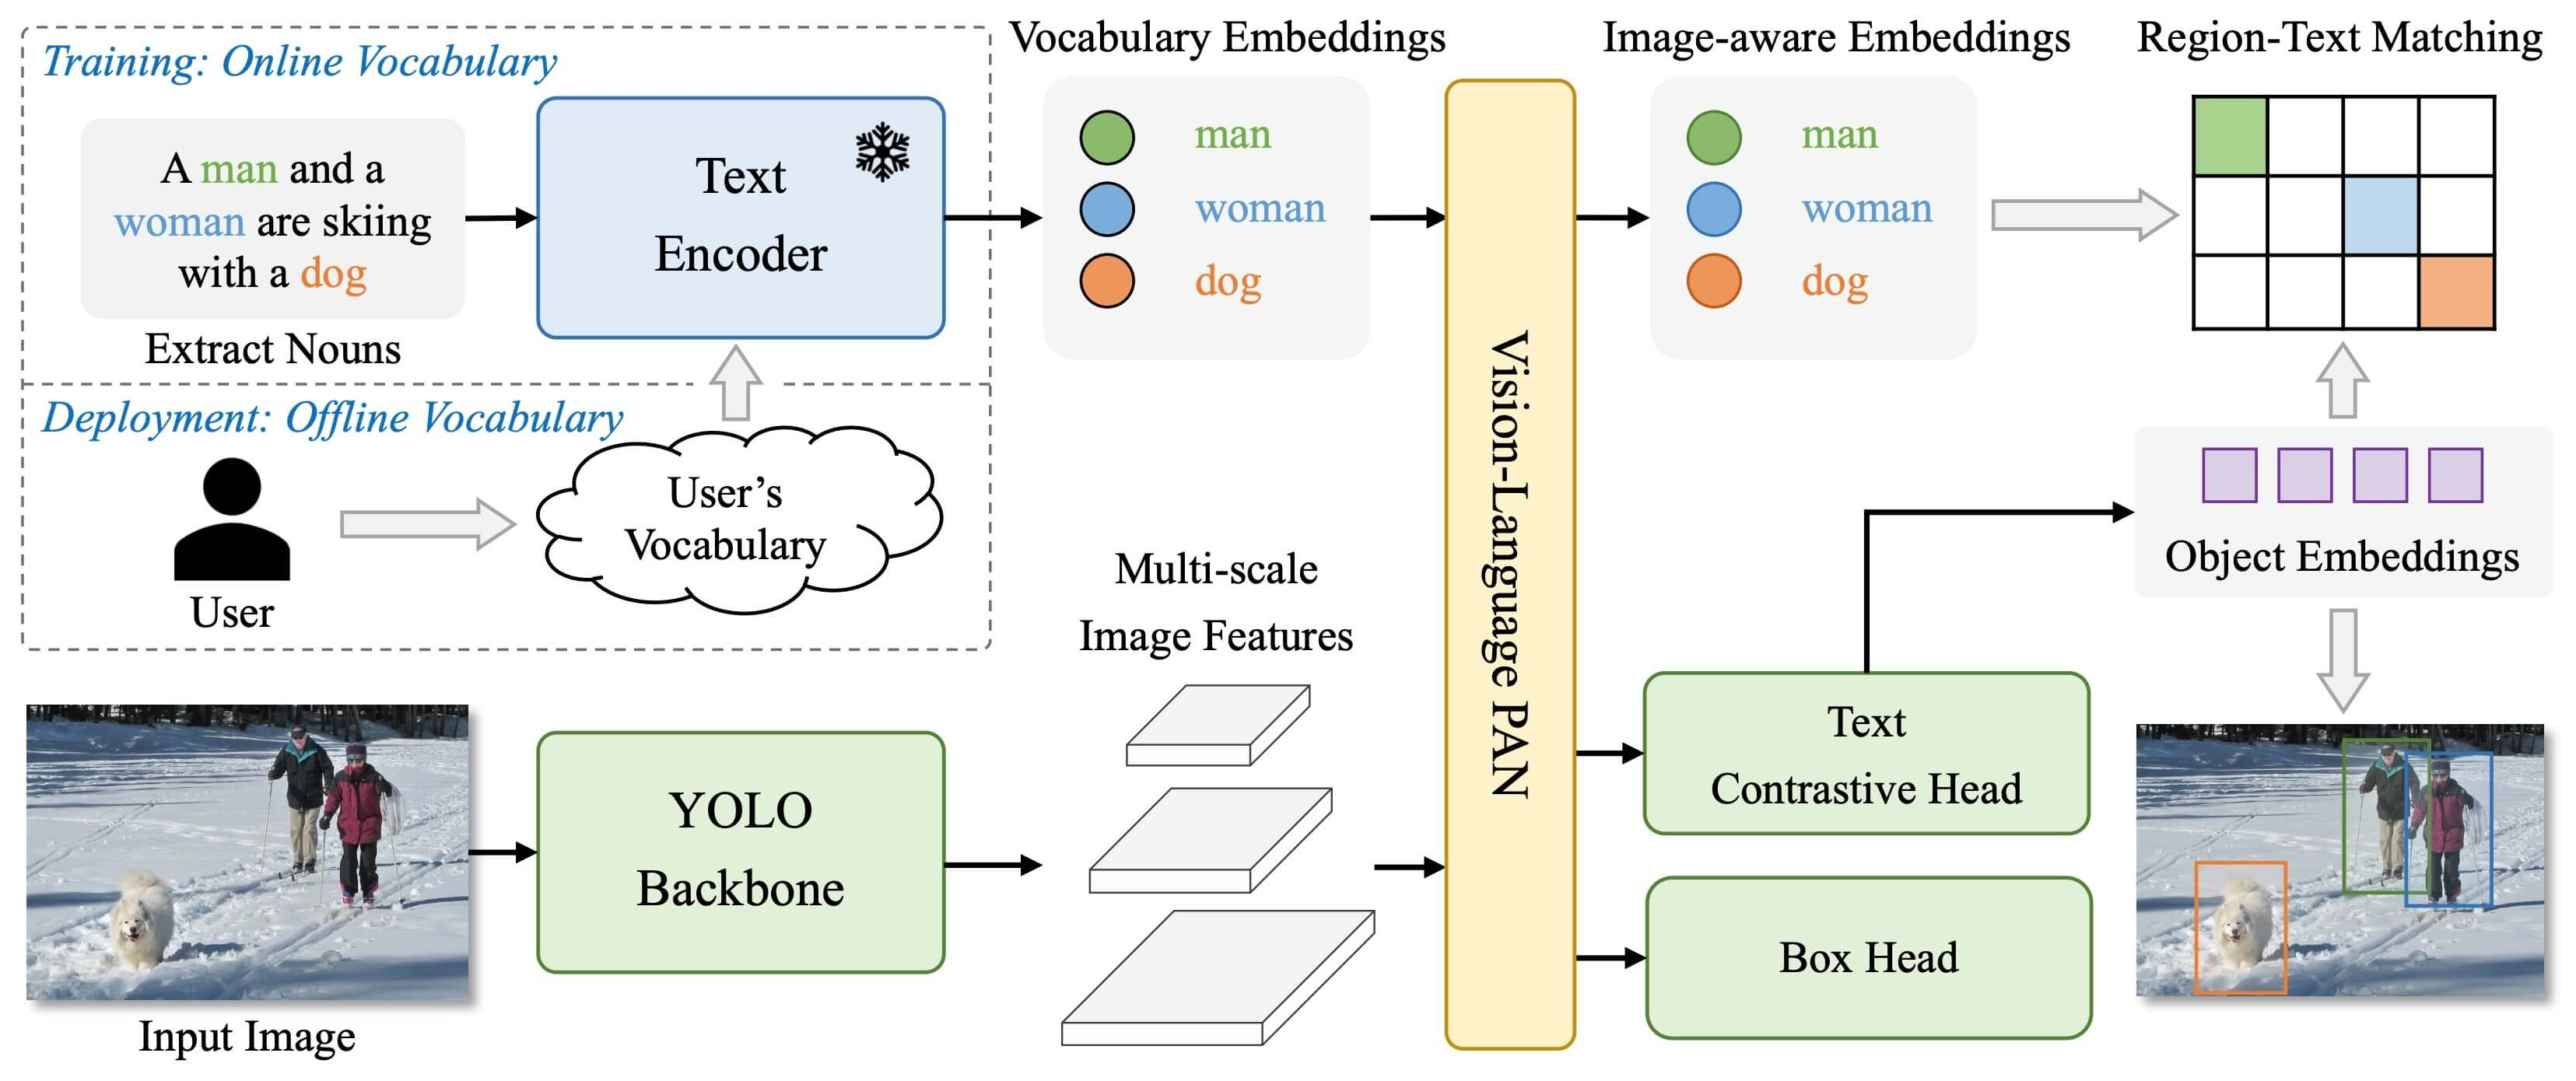
\includegraphics[width=1\textwidth]{files/capitoli/2-yolo/assets/yoloworld-architecture.jpeg}
    \caption{\label{fig:yoloworld-architecture}Architettura di YOLO-World\cite{30}}
\end{figure}

\newpage

\subsection{RT-DETR}
RT-DETR, o Real-Time DETR, è un'evoluzione del modello DETR (DEtection TRansformer) sviluppato da Baidu\cite{31}, che mira a migliorare le prestazioni di object detection in tempo reale.

\subsubsection{Caratteristiche principali}
Le principali caratteristiche del modello RT-DETR sono:
\begin{itemize}
  \item \textbf{Efficient Hybrid Encoder}: incorpora un encoder che sfrutta i Vision Transformers (ViT) per gestire efficientemente le feature multiscala, permettendo così al RT-DETR di acquisire una comprensione globale delle immagini, migliorando la capacità di rilevamento degli oggetti senza dipendere esclusivamente da filtri locali come nelle CNN.
  \item \textbf{Selezione delle Query consapevole dell'IoU}: migliora l'inizializzazione delle query degli oggetti attraverso una selezione consapevole dell'indice di sovrapposizione (IoU), permettendo al modello di concentrarsi sugli oggetti più pertinenti della scena e migliorando l'accuratezza della detection.
  \item \textbf{Velocità di Inferenza Adattabile}: offre flessibilità nella regolazione della velocità di inferenza utilizzando diversi strati del decoder senza necessità di riaddestramento
\end{itemize}

\subsubsection{Architettura}
L'architettura di RT-DETR consiste sempre in 3 componenti principali:
\begin{itemize}
  \item \textbf{Backbone}: utilizza un approccio innovativo il quale non si limita alla selezione delle feature map finali del backbone, bensì utilizza feature provenienti da tre diversi livelli diversi di quest'ultimo. Gli stadi S3, S4 e S5 del backbone vengono impiegati come input per l'encoder, fungendo così da estrattore di caratteristiche multiscala per il modello.
  \item \textbf{Efficient Hybrid Encoder}: trasforma le feature in una sequenza di feature dell'immagine, utilizzando due altri moduli:
  \begin{itemize}
    \item \textbf{AIFI (Attention based Intra Scale Feature Interaction)}, il quale si occupa esclusivamente della feature map S5 per estrarre interpretazioni semantiche più elaborate, aumentando l'accuratezza complessiva.
    \item \textbf{CCFM (CNN based Cross-scale Feature-fusion Module)}, che estrapola interpretazioni semantiche sia da S4 che da S5, ed incorpora un Fusion Block che fonde le caratteristiche di due blocchi adiacenti in una nuova feature.
  \end{itemize}
  \item \textbf{IoU Aware Query Selection e Transformer Decorder}: il primo è il modulo adibito alla selezione delle feature in base all'indice di sovrapposizione, le quali serviranno da input per il decoder, responsabile della generazione delle bounding box e dei punteggi di confidenza.
\end{itemize}

\begin{figure}[ht]
    \centering
    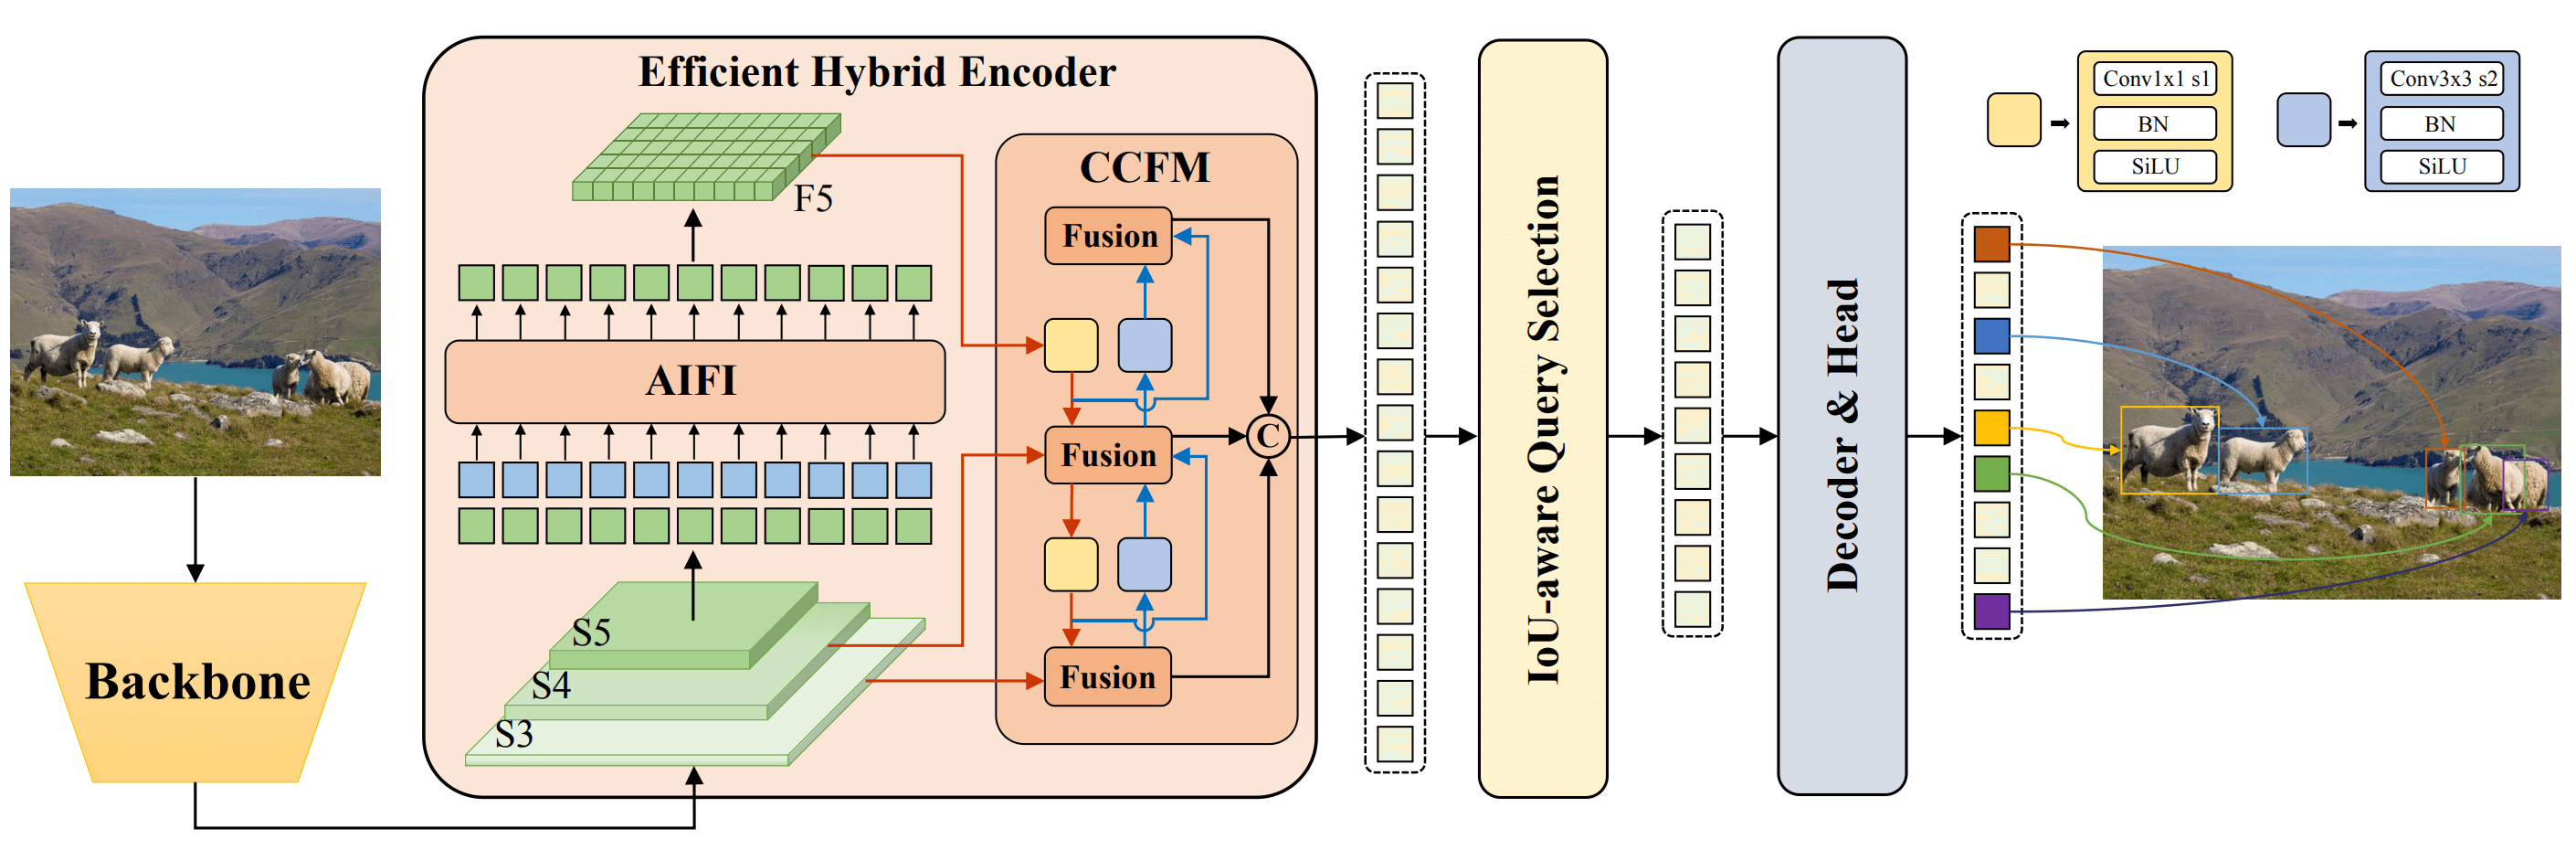
\includegraphics[width=1\textwidth]{files/capitoli/2-yolo/assets/rtdetr-architecture.png}
    \caption{\label{fig:rtdetr-architecture}Architettura di RT-DETR\cite{32}}
\end{figure}
